\section{Habib Abdul Rasyid (1174002)}
\subsection{Pengertian}
Sistem Informasi Geografis terdiri atas 3 kata. Yaitu Sistem, Informasi, dan Geografis.
\begin{itemize}
	\item SISTEM \break
Definisi sistem secara umum adalah unit yang terdiri dari komponen atau elemen yang saling berinteraksi, saling terkait, atau saling tergantung untuk membentuk keseluruhan yang kompleks.
	\item INFORMASI \break
Informasi adalah data yang telah diolah menjadi bentuk yang memiliki makna bagi penerimanya dan bisa dalam bentuk fakta, nilai-nilai bermanfaat. Pada bagian ini terdapat proses transformasi data menjadi informasi, yaitu proses input-output.
	\item GEOGRAFI \break
Geografi adalah studi tentang lokasi dan persamaan dan perbedaan variasi spasial dalam fenomena fisik dan manusia di permukaan bumi. Definisi lain dari geografi adalah studi tentang persamaan dan perbedaan dalam fenomena geologis dari perspektif regional dan lingkungan dalam konteks spasial.
	\item SISTEM INFORMASI \break
Pengertian Sistem informasi secara umum adalah sistem terintegrasi yang mampu memberikan informasi yang bermanfaat bagi penggunanya, memberikan informasi untuk mendukung operasi, manajemen dalam suatu organisasi. Sistem ini menggunakan perangkat keras dan lunak komputer, prosedur manual, model manajemen, dan basis data
	\item SISTEM INFORMASI GEOGRAFIS \break
Pengertian Sistem Informasi Geografis (SIG) secara umum adalah sistem informasi khusus yang digunakan untuk mengelola data yang memiliki informasi geospasial. GIS juga merupakan jenis perangkat lunak yang dapat digunakan untuk mengimpor, menyimpan, memanipulasi, menampilkan, dan mengeluarkan informasi geografis dan atributnya. GIS digunakan untuk memberikan nilai, dengan mengatur dan menampilkan data secara tepat, menggabungkannya dengan data lain, menganalisis data, dan menghasilkan data baru yang bermanfaat, pada gilirannya GIS dapat membantu untuk pengambilan keputusan. Sistem Informasi Geografis dibagi menjadi dua kelompok, yaitu sistem manual (analog), dan sistem otomatis (yang didasarkan pada komputer digital). Perbedaan paling mendasar terletak pada cara pengelolaannya.
\end{itemize}


\subsection{Sejarah}
Pada awal 1960-an perkembangan ilmu komputer berkembang pesat dan siap digunakan untuk bidang lain di luar militer. Ahli meteorologi, geologi dan geofisika mulai menggunakan komputer dalam membuat peta.
Pada tahun 1963 di Kanada, CGIS (Sistem Informasi Geografis Kanada) muncul, dan kemudian menjadi GIS pertama di dunia. Dua tahun kemudian di Amerika Serikat mengoperasikan sistem serupa yang disebut MIDAS yang digunakan untuk memproses data sumber daya alam.
Seiring dengan perkembangan teknologi, GIS juga telah berubah menjadi lebih baik. Berikut ini adalah sejarah perkembangan SIG dari waktu ke waktu:
\begin{itemize}
	\item35.000 tahun lalu, di dinding gua Lascaux, Prancis, pemburu Cro-Magnon menggambar hewan mangsa mereka, serta garis yang diyakini sebagai rute migrasi hewan-hewan. Catatan awal ini sejalan dengan dua elemen struktural dalam sistem informasi geografis modern saat ini, arsip grafik yang terhubung ke database atribut.
	\item Pada 1700-an, teknik survei modern untuk pemetaan topografi diterapkan, termasuk versi awal pemetaan tematik, misalnya untuk data ilmiah atau sensus.
	\item Awal abad ke-20 menyaksikan perkembangan "foto litograf" di mana peta dipisahkan menjadi beberapa lapisan. Perkembangan perangkat keras komputer yang didorong oleh penelitian senjata nuklir membawa aplikasi pemetaan ke multifungsi pada awal 1960-an.
	\item 1967 adalah awal dari pengembangan GIS yang dapat diimplementasikan di Ottawa, Ontario oleh Departemen Energi, Tambang dan Sumber Daya. Dikembangkan oleh Roger Tomlinson, yang kemudian disebut CGIS (GIS Kanada - GIS Kanada), digunakan untuk menyimpan, menganalisis, dan memproses data yang dikumpulkan untuk Inventarisasi Tanah Kanada (CLI - inventaris tanah Kanada) - sebuah inisiatif untuk mengetahui kemampuan lahan di pedesaan Kanada dengan peta. berbagai informasi tentang tanah, pertanian, pariwisata, liar, unggas dan penggunaan lahan pada skala 1: 250000. Klasifikasi faktor peringkat juga diterapkan untuk analisis.
	\item GIS dengan gvSIG.CGIS adalah sistem pertama di dunia dan hasil dari aplikasi pemetaan yang disempurnakan yang memiliki kemampuan untuk melapisi, menghitung, mendigitalkan / memindai, mendukung sistem koordinat nasional yang memanjang melintasi benua Amerika, memasukkan garis sebagai busur dengan atribut topologi dan toko dan informasi lokasi dalam file terpisah. Pengembang, seorang ahli geografi bernama Roger Tomlinson, kemudian dipanggil "Mr. GIS".
	\item CGIS bertahan hingga tahun 1970-an dan membutuhkan waktu lama untuk membaik setelah pengembangan awal, dan tidak dapat bersaing dengan aplikasi pemetaan komersial yang dirilis oleh vendor seperti Intergraph. Pengembangan perangkat keras komputer mikro mendorong vendor lain seperti ESRI dan CARIS untuk membuat banyak fitur GIS, menggabungkan pendekatan generasi pertama dengan pemisahan informasi spasial dan atribut, dengan pendekatan generasi kedua pada organisasi data atribut ke dalam struktur basis data. Pengembangan industri pada 1980-an dan 1990-an semakin memacu pertumbuhan GIS pada workstation UNIX dan komputer pribadi. Pada akhir abad ke-20, pertumbuhan yang cepat di berbagai sistem dikonsolidasikan dan distandarisasi ke dalam platform yang lebih sedikit, dan pengguna mulai mengekspor tampilan data GIS melalui internet, yang membutuhkan standar pada format dan transfer data.
\end{itemize}



\subsection{Koordinasi}
Untuk menggambarkan permukaan bumi yang berbentuk seperti bola menjadi bentuk peta, kita membutuhkan persamaan matematika yang dapat membantu mengubah citra permukaan bumi. Persamaan ini disebut sistem koordinat. Koordinat adalah karakteristik utama SIG karena sistem koordinat ini dapat menunjukkan referensi geografis pada data SIG. Dapat dikatakan bahwa sistem koordinat adalah pendekatan dalam mendefinisikan posisi data SIG di permukaan bumi.
Dalam sistem koordinat, posisi benda di permukaan bumi ditentukan oleh garis lintang dan bujur. Latitude adalah garis horizontal yang mengukur sudut antara titik dan khatulistiwa (khatulistiwa). Sedangkan garis bujur adalah garis vertikal yang mengukur sudut suatu titik dengan titik nol bumi, yaitu Greenwich Meridian, London
Lintang dibagi menjadi 2, yaitu lintang utara dan selatan dan bujur dibagi menjadi bujur timur dan bujur barat. Sumbu x sebagai garis lintang dan sumbu y sebagai garis bujur dalam koordinat Cartesius.

\subsection{Geospasial}
Data geospasial adalah data tentang aspek fisik dan administrasi dari suatu objek geografis. Aspek fisik yang dimaksud meliputi bentuk-bentuk antropogenik dan alami baik di permukaan maupun di bawah permukaan bumi. Bentuk antropogenik mengandung fenomena budaya seperti jalan, rel kereta api, bangunan, jembatan, dan sebagainya. Tentu saja alam adalah sungai, danau, pantai, dataran tinggi, dan sebagainya. Sedangkan aspek administratif adalah batas distribusi atau sosial-budaya yang dibuat oleh suatu organisasi atau lembaga dengan tujuan mengatur dan menggunakan sumber daya alam. Termasuk dalam aspek perbatasan negara, pembagian wilayah administratif, zona, kode pos, batas kepemilikan tanah, dan sebagainya.
Secara umum ada dua metode untuk menampilkan fitur geografis ke GIS atau Sistem Informasi Geospasial. Pertama, struktur data vektor (struktur data vektor) terdiri dari deskripsi titik geografis, dalam bentuk titik, garis, atau poligon. Model grafik vektor ini menampilkan fitur geografis terpisah seperti batas administratif, jalan, bangunan, dan sungai. Objek grafis biasanya dikaitkan dengan informasi yang berisi penjelasan tentang atribut objek, dan informasi ini dapat disimpan dalam spreadsheet atau file database yang terpisah. Kedua, struktur data raster terdiri dari serangkaian sel atau piksel yang biasanya digunakan untuk menggambarkan data gambar sebagai data kontinu. Dalam struktur data seperti itu, ada unsur resolusi sebagai ukuran dimensi fitur geografis yang direpresentasikan dalam bentuk piksel. Biasanya data raster ini digunakan untuk citra satelit, ortografi digital, model elevasi digital, peta digital.

\subsection{Link}
\href{https://youtu.be/zhZPF4EKivU}{https://youtu.be/zhZPF4EKivU}

\subsection{Plagiarism}
\begin{figure}[H]
	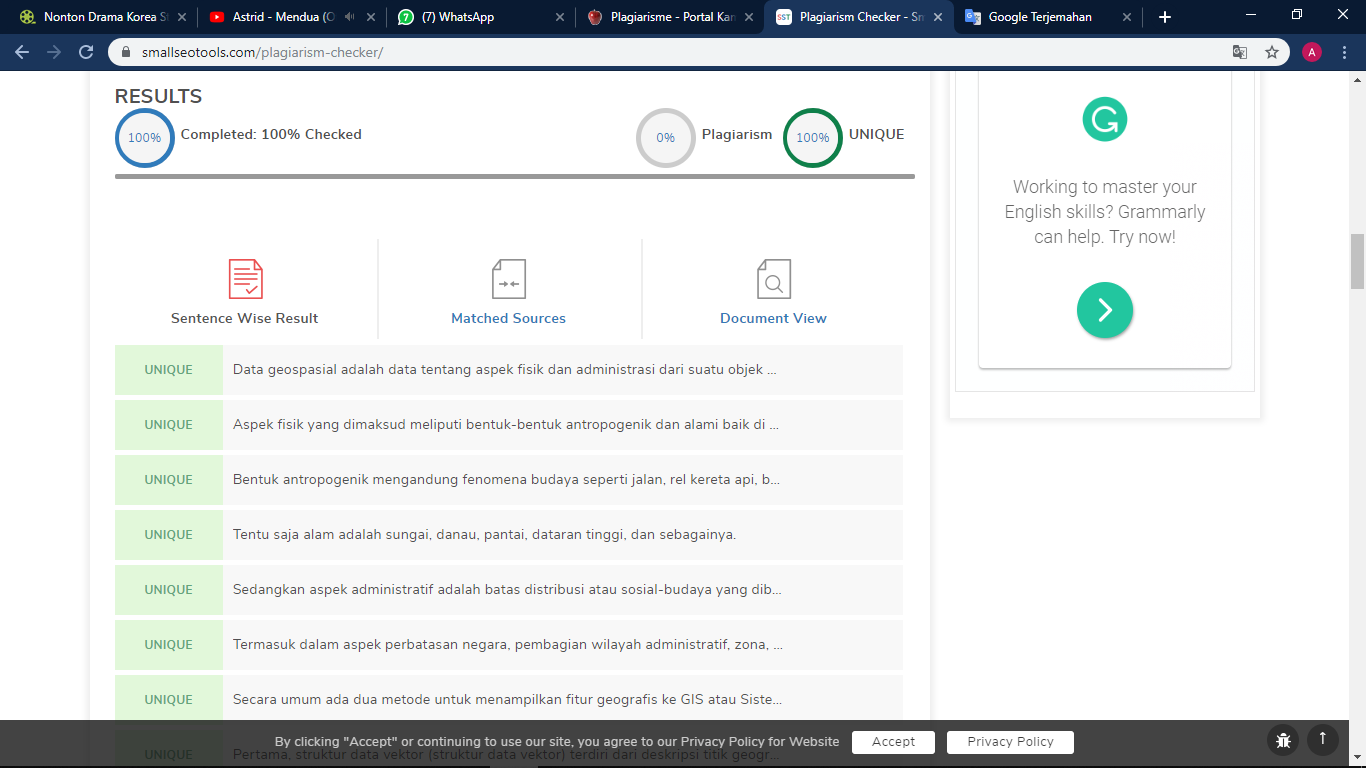
\includegraphics[width=4cm]{figures/1174002/SSGIS.png}
	\centering
	\caption{Plagiarism 1174002}
\end{figure}
